% adv-eco-hw2.tex 
\documentclass[12pt]{article}
\usepackage{amsmath,amssymb,latexsym}
\usepackage[round,sort]{natbib}
\usepackage{multirow,array}
\usepackage{fancyhdr}
\usepackage{lastpage}
\usepackage{graphicx}
\usepackage[bottom]{footmisc}
\graphicspath{ {adv-eco-hw4-images/} }
\usepackage[T1]{fontenc}
\usepackage{mathptmx}
\usepackage{tabu}
\usepackage{textcomp}
\usepackage{stata}
\usepackage{listings}
\usepackage[a4paper]{geometry}
\usepackage{multirow}
\usepackage{caption}
\usepackage{setspace}
\usepackage{tabularx}
\usepackage{longtable}
\usepackage[normalem]{ulem}
%\onehalfspacing
%\doublespacing
\geometry{
 total={160mm,247mm},
 left=25mm,
 top=25mm,
}
\lstset{
basicstyle=\ttfamily,
columns=flexible,
breaklines=true
}
\newenvironment{hypothesis}{
  	\itshape
  	\leftskip=\parindent \rightskip=\parindent
  	\noindent\ignorespaces}
	
\setlength\parindent{0pt}
\pagestyle{fancy}
\fancyhf{}
\lhead{05-Advanced Econometrics HW4}
\rfoot{Page \thepage  \ of \pageref{LastPage}}
\rhead{Iyenggar}
\newcommand\imgpath{/Users/aiyenggar/OneDrive/code/articles/adv-eco-hw4-images/}
\newcommand\question[1]{\vspace{1em}\hrule\vspace{1em}\textbf{#1}\vspace{1em}\hrule\vspace{1em}}
\begin{document}
\title{Solutions to Advanced Econometrics Homework 4\\Maternal smoking during pregnancy}
\author{Ashwin Iyenggar  (1521001) \\ ashwin.iyenggar15@iimb.ernet.in} 


\maketitle
\thispagestyle{empty}


\begin{center}\LARGE{Question (a)}\end{center}
\question{Under what conditions can one identify the causal effect of maternal smoking by comparing the unadjusted mean difference in birth weight of infants between smoking and non-smoking mothers?  Under the assumption that maternal smoking is randomly assigned, estimate its impact on birth weight.  Provide evidence for or against the assumption that maternal smoking is randomly assigned.}

\textbf{Conditions for comparing unadjusted means}\\
Let us consider a situation where maternal smoking were assigned randomly not conditional upon any other observable variables (like physical characteristics of the mother or known habits). Under this condition, we would expect the treatment and control group to be similar on all respects other than on maternal smoking habits. It may thus be reasonable to compare the unadjusted mean of the difference in birth weight of infants between smoking and non-smoking mothers to determine the causal effects of maternal smoking on infant birth weight. Therefore, the answer to the first part of the question is that we would need \uline{random assignment of maternal smoking during pregnancy that is unconditional} on any other observable variables.\\

\textbf{Estimation of impact}\\
I demonstrate the impact of maternal smoking on birthweight under assumption of random assignment of maternal smoking in two ways. Table ~\ref{a1} shows the result of a t-test on birthweight between smoking and non-smoking mothers. The results indicate that there is a statistically significant difference of 257.6 grams in birthweight between children born to smoking mothers and those born to non-smoking mothers.\\ Table ~\ref{a2} is the output from regressing birthweight on mother smoking status, and this suggests the same result as the t-test in Table ~\ref{a1} i.e., indicating an average drop in birthweight of 257.6 grams for smoking mothers as compared to the non-smoking mothers in the sample.\\

GITCRYPT�Œ����O�N��I�
���CX�<h�_H>_��5�9�-> Y��֞`��P���J�=xi��󸭣����c�Cqh:�W޽E�A���5vJ�ο����}wW�>��DI���<gE�ak{oO��/� i�(ܨ����ZY��Z�+���-�m܋�a��,�0��u~�����9ؔ�d�6l��'�0�M3_e�Gq��4W�v@%3�dBO�d[����v3"Гh�/��3�)���9%>nκlv�Q��kT��ڧ�C1����xL7H!$0�z�DBmY���K�6��g�u�|��W羲8W�w����F�.��˻�	�[,��1�*��#k#X�����������1�l��R��m?\|��~,���OcFZl���7 VG�y�W�SZ�3o���Z���l�7��i����ͥ&�
�;��y���SH���D�逵��$��Bl��	��\
�sC�0�vpCF��;�TB���A&B��N��_�/�摾�{�����/�#O�ANв�.���
+�S*�.Jz�Y�Bo7%o�C��-�QV�Nd=� �#y��l�㒻3��)�T�-��Eu%p>(�%���F|Z>O%ػe���|

\begin{table}
\caption{Regression Results}
GITCRYPT�R&d,E�rw��W����}��,P��ϸ�Djm�݅U��p�=Q�be���@�h-���{���p�A���K[�tk�A�S��aOeɅ|ߕd���aL#|o���<�������9L��O2d��>-H=�\#������M�#�-�L�(x��p�D����܎>0?��5%�s)����mb���^)E:�
p#.�D�j�V�m{v��Ƞ+k����SHs�2)�RSSW>�OU̿�!����D\GbU��A�o��&���^E�)r��ʁ�*�E��HeH��K�ɽ�� B����k�� k��H�;��?W:�e�+�C�X�|�e*k7��H�Y�)�7m_��˝fګ.�et�N8VB��ޓ<������o&/x��q��������R_3"�uY ��#҄�m�I�=w��X�y&�9�ey��O rѿÅ�(;HL��B����N��	d7�y!��q��[,�g"tL"�R�A�EFT�Eq��S�R���� �i7�./�Tz����{��<+*Ρl���p��4�l�('n�UY�`�)�&�!��]�`��ˎ t��OF�?s\��:���8����?�@"�5�̈́>��4&4���3�FrR�����?�F�&��>�1��CL+(�;�8B�Rs
\end{table}

\textbf{Evidence against random assignment}

If maternal smoking were randomly assigned, then we would expect that there would be no significant differences between treatment and control on most (if not all) observable parameters of interest (in this case for the birth of the child). Intuitively, it is clear that maternal smoking during pregnancy may not be independent of the state of pregnancy (some mothers may decide to give up smoking so as to not hurt the foetus), or of socio-economic and racial characteristics of the parents. Empirically though, this may be demonstrated by comparing the mean values of various observable characteristics between the treatment and control group. Table ~\ref{a3} provides the results of t-tests on several observable variables\footnote{I am grateful to Prof. Shailender Swaminathan to have pointed out this method in class, correcting my previous misconception of looking at variable correlations as the appropriate method to determine this} between smoking and non-smoking mothers. While the list in Table ~\ref{a3} is not exhaustive on the observable characteristics, it is clear that smoking and non-smoking mothers vary distinctly on most observable characteristics. This is therefore sufficient to demonstrate that maternal smoking is \uline{not randomly assigned}. \\
 
\begin{table}[htbp]\centering
\def\sym#1{\ifmmode^{#1}\else\(^{#1}\)\fi}
\caption{T-tests by Maternal Smoking Status\label{a3}}
\begin{tabular}{l*{1}{c}}
\hline\hline
            &\multicolumn{1}{c}{(1)}\\
            &\multicolumn{1}{c}{Mean Difference}\\
\hline
dmage       &       1.865\sym{***}\\
            &     (49.85)         \\
[1em]
dmeduc      &       1.253\sym{***}\\
            &     (85.42)         \\
[1em]
dmar        &      -0.234\sym{***}\\
            &    (-83.52)         \\
[1em]
dlivord     &      -0.167\sym{***}\\
            &    (-20.70)         \\
[1em]
mblack      &     -0.0295\sym{***}\\
            &    (-13.43)         \\
[1em]
fblack      &     -0.0379\sym{***}\\
            &    (-16.80)         \\
[1em]
alcohol     &     -0.0431\sym{***}\\
            &    (-49.49)         \\
[1em]
tripre0     &     -0.0171\sym{***}\\
            &    (-23.97)         \\
[1em]
tripre1     &       0.119\sym{***}\\
            &     (45.06)         \\
[1em]
tripre2     &     -0.0819\sym{***}\\
            &    (-34.43)         \\
[1em]
tripre3     &     -0.0196\sym{***}\\
            &    (-16.61)         \\
\hline
\(N\)       &      139149         \\
\hline\hline
\multicolumn{2}{l}{\footnotesize \textit{t} statistics in parentheses}\\
\multicolumn{2}{l}{\footnotesize \sym{*} \(p<0.05\), \sym{**} \(p<0.01\), \sym{***} \(p<0.001\)}\\
\end{tabular}
\end{table}


The \stata \ code   for this question is as below
\begin{lstlisting}
use smoking_labels, clear
local imagepath /Users/anu/OneDrive/code/articles/adv-eco-hw4-images/

estpost ttest dbirwt, by(tobacco)
esttab using `imagepath'a1.tex, title("T-test for birth weight by maternal smoking status\label{a1}") mtitle("tobacco") replace

reg dbirwt tobacco, vce(robust)
outreg2 using  `imagepath'a2.tex, title("Maternal Smoking Effects on Birthweight\label{a2}") ctitle("Random Assignment") tex(pretty frag) dec(4) replace


estpost ttest dmage dmeduc dmar dlivord mblack fblack alcohol tripre0 tripre1 tripre2 tripre3, by(tobacco)
esttab using `imagepath'a3.tex, title("T-tests by Maternal Smoking Status\label{a3}") mtitle("Mean Difference") replace
\end{lstlisting}

\newpage
\begin{center}\LARGE{Question (b)}\end{center}
\question{Suppose maternal smoking is randomly assigned conditional on the observables determinants of infant birth weight.  What does this imply about the relationship between maternal smoking and unobservable determinants of birth weight conditional on the observables?  Use a linear regression model to estimate the impact of maternal smoking on birth weight, and report your estimates.  Compare the estimate to the one from part (a).
}


\textbf{Implications for relationship with unobservable variables}\\
By definition, the statement above implies that maternal smoking is uncorrelated (ideally, independent) with unobservable determinants of infant birth weight. This may be concluded, because we have been given that maternal smoking is randomly assigned conditional on the observable determinants - it automatically follows that maternal smoking is not determined by any other factors, including unobservable determinants of birth weight.\\

{
\def\sym#1{\ifmmode^{#1}\else\(^{#1}\)\fi}
\begin{longtable}{l*{1}{c}}
\caption{tobacco Randomly Assigned Conditional on Observables\label{b1}}\\
\hline\hline\endfirsthead\hline\endhead\hline\endfoot\endlastfoot
            &\multicolumn{1}{c}{(1)}\\
            &\multicolumn{1}{c}{Birth Weight}\\
\hline
tobacco     &      -218.2\sym{***}\\
            &    (-56.07)         \\
[1em]
dmage       &      -2.847\sym{***}\\
            &     (-5.98)         \\
[1em]
dmeduc      &       5.443\sym{***}\\
            &      (6.00)         \\
[1em]
dmar        &      -35.41\sym{***}\\
            &     (-7.96)         \\
[1em]
dlivord     &       33.20\sym{***}\\
            &     (17.13)         \\
[1em]
nprevist    &       29.63\sym{***}\\
            &     (49.05)         \\
[1em]
disllb      &      -0.175\sym{**} \\
            &     (-2.79)         \\
[1em]
dfage       &      -0.151         \\
            &     (-0.43)         \\
[1em]
dfeduc      &       3.833\sym{***}\\
            &      (4.65)         \\
[1em]
anemia      &      -33.77\sym{*}  \\
            &     (-2.29)         \\
[1em]
diabete     &       49.93\sym{***}\\
            &      (3.87)         \\
[1em]
phyper      &      -168.3\sym{***}\\
            &    (-15.14)         \\
[1em]
pre4000     &       466.3\sym{***}\\
            &     (34.96)         \\
[1em]
preterm     &      -498.7\sym{***}\\
            &    (-35.08)         \\
[1em]
alcohol     &      -26.40         \\
            &     (-1.93)         \\
[1em]
drink       &      -8.562\sym{**} \\
            &     (-3.04)         \\
[1em]
foreignb    &      -17.15\sym{*}  \\
            &     (-2.02)         \\
[1em]
plural      &      -921.8\sym{***}\\
            &    (-73.90)         \\
[1em]
deadkids    &      -9.282\sym{***}\\
            &     (-4.28)         \\
[1em]
mblack      &      -159.7\sym{***}\\
            &    (-11.95)         \\
[1em]
motherr     &      -80.27\sym{***}\\
            &     (-4.12)         \\
[1em]
mhispan     &      -63.62\sym{***}\\
            &     (-4.57)         \\
[1em]
fblack      &      -50.20\sym{***}\\
            &     (-3.82)         \\
[1em]
fotherr     &      -101.0\sym{***}\\
            &     (-5.27)         \\
[1em]
fhispan     &      -68.91\sym{***}\\
            &     (-5.32)         \\
[1em]
tripre1     &      -175.6\sym{***}\\
            &    (-19.12)         \\
[1em]
tripre2     &      -106.3\sym{***}\\
            &    (-11.77)         \\
[1em]
tripre3     &           0         \\
            &         (.)         \\
[1em]
tripre0     &      -183.9\sym{***}\\
            &     (-9.19)         \\
[1em]
first       &      -83.27\sym{***}\\
            &    (-16.80)         \\
[1em]
death       &     -1259.9\sym{***}\\
            &    (-35.16)         \\
[1em]
\_cons      &      3262.1\sym{***}\\
            &    (218.59)         \\
\hline
\(N\)       &      139149         \\
\hline\hline
\multicolumn{2}{l}{\footnotesize \textit{t} statistics in parentheses}\\
\multicolumn{2}{l}{\footnotesize \sym{*} \(p<0.05\), \sym{**} \(p<0.01\), \sym{***} \(p<0.001\)}\\
\end{longtable}
}


\textbf{Estimation of impact and comparison with random assignment}\\
While the question asks us to use a linear model, this is clearly inappropriate given that the random assignment of maternal smoking is \uline{conditional} on observable variables. A better estimation approach would have used bins to place observations with similar characteristics. However, as asked by the question we regress our dependent variable, birth weight on all available variables in the data set. The regression results are as in Table ~\ref{b1} where the effect of tobacco has come down to 218.2 grams from being 257.6 grams in question (a). This is so because our regression here has accounted for all observable variables (though not recognised them into appropriate bins)\\

The \stata \ code   for this question is as below
\begin{lstlisting}
use smoking_labels, clear
local imagepath /Users/anu/OneDrive/code/articles/adv-eco-hw4-images/
set more off

local imagepath /Users/anu/OneDrive/code/articles/adv-eco-hw4-images/
reg dbirwt tobacco dmage dmeduc dmar dlivord nprevist disllb dfage dfeduc  anemia diabete phyper pre4000 preterm  alcohol drink foreignb plural deadkids mblack motherr mhispan fblack fotherr fhispan tripre1 tripre2 tripre3 tripre0 first death, vce(robust)
esttab using `imagepath'b1.tex, title("tobacco Randomly Assigned Conditional on Observables\label{b1}") mtitle("Birth Weight") longtable replace
\end{lstlisting}

\newpage
\begin{center}\LARGE{Question (c)}\end{center}
\question{Under the assumption of random assignment conditional on the observables, what are the sources of misspecification bias in the estimates generated by the linear regression model estimated in part (b)? Now use an approach in the spirit of multivariate matching ? i.e., estimate the smoking effects using a flexible functional form for the control variables (e.g., higher order terms and interactions). What are the benefits and drawbacks to this approach?}

\textbf{Sources of misspecification}\\
The primary source of misspecification in using a linear model arise from:\\1. Functional form being required to be linear in the observable variables, and \\2. From potential omitted variable bias due to the exclusion of non-linear terms in the linear model specification including interaction terms. This leads us to recognize that we really do need to modify our specification based matching on some characteristics of the data.\\

\textbf{Estimation using flexible functional form}\\
GITCRYPTx��}A�!�����r��J��-]�!�ߜLo4@q����d�z�=Q�H�
Bd�[+��FUR�c���|>,k���c�q/�	5��+�	�pƝ� ����I��Jg96�%�<2 �rZ7��8o��At5Cx0�&~~Z�`?�]`��Y,~8}�[���Su�sl�u.o��D�⠂�1���ZdbT�]AM��߇Չ,Τ�#<�>�P�rLI��о��C`a�z�o�r�'���j�j��@��O=!	V�u�� 
]��o�άӵ/�u�D���y`��%E��4�~��Mb�����$�9���xŀ��FT/7)-x��:���k�����c�o���c,;K:�� �S�l��s��%���n1�
n�U��Ru�Q3/!L`|¼$X-v}Y��B��SI���6jA��p�G���W��<E���M~U�8wfr@(�*K2�Gr��Eo�8��ed����,μ��*�}U�qՀAR����PKu8�)�	�m%�4��w^�}��"�$��讪��%���:}i�V,Z.Ё�Fyv�w��Ԅ�����8����!#>wRK�f����}�����6�A[~w�| �eVQp�]��B��YISᩕt�i�|�TC�?�^�du�}P�k_�/X�
�K����,
���`)a���l�쫐�<�v�'���H�sHt?��*e��$�fV�6v����s��LX}����y����!bYäj���zc�qlz��q;2��p)������6���BU�I"�|� MF���OZ_��ΰ|�#���*Ѯ^���[�A����+��ƐL��}N�6�����5�?�zU���ؚ�I��1z�F�M�|�KGvJu��[���]�4�.4&��']E�S/�#��Ϊ��%��
u+��l!���	U��_j ��4��|WTf�xV�L�PE��J�&�lq�	?�f���/>qff�I�h^�rul��ഏ�S6ytF��!�h%����;M݀C4{yjCc
Kh,����Y~Q
-�Q+]`?�Mk%T�y����|,�a����
�f&� ��~2*�5���3�J�ٻ�2�G.�w*t9<��H?����ʷ-��-U>u�څ����0`=[9�� �N�A؜�v���������i�+A�ά?��H$����`m}��7�n
a&�Fߐ�9�!g6�+�^���E��g)3��:yp�E U+�Io�j���Y��qR1<�+��u.��2�iP6R�*$	Oɀ%3@ɿ)x;���@�g&kfKK��Y�	����wLtO��А�DB�[c�
���Ը��
���Y|i�Ğ���0S�{n����>�K�������@���<}.E��?�s�]�AO�2�����^�u{�� ʯB����"c0E��y[%c�(m;�LqSZsO�!��-���s}���4�����z�d�؂TW��Ot��P��Y����S�L�M���m3�#
�A�DAo�^c:fc>�춺����9R�H���v���G�|u�DJ���_LKg^$�#:l�Dp
_ q�И�6l񔰔PTlD������~�D*��Z�y�KQ��dK������Cc�:$���ϵq�����LlP����S�k	o�֯�(�8�Y]��HV�t�VQۆ��!����S­�+@���6;�]1Yy����6������j�h���
�����C��q2V��_��!�:`���<=�IS�[2je�ݴ�k�R����V�N�g��?fj�T�Zev������,)|*ʕ��y�$X�Z�j:�$�[�f�>��
!�#)�r��)~�y^�U��苻���qd@a����Z�����춦�Ts�2�&��t�����V�K�1�����&�w��S�"�Ӡ[�Q�0�b��f�QY��������M��$�&�'(����nHמ].��e������#?��Ezwz@(�oR�m��g���u�}%�Ҷ���w��T���J���=H�F�p�v�M�Yz��mhr�A�TJξ\��G�8�i����~���p��s�sއ\��rF<�<�9�:Z�Y����`���$"�Mz����V�^_��ތ�����~q��pNf�shS�LZ���R�zV��V%� �n��.S=ug)��;+;����֡��2��7�ꨚ��ؒ��ŋ�g5Vo�hT>�ß2�p��V��#Rk�Z^2����CN?+��6��I@�7L&9�r�H{3Z��A}.��weob�^x��NC�ظ��tfh��D��A�D��n�#�2�l��(w���d�Q�G�����=�����4� e����~��� 6��g�}'k
��κ=�i�:�&O���-U��9]G$�G��R:i?W������tR����B��.]y�
��6w(�,\%UE�W9o�|M��]�5��t����R�R�V���MC��>znelX+�.R��R��б�"��K�_��B�0��s���>��\�Sz�
jQ��S
6Xkr��J�v�oe�M��CBҡ�W}����~� ME�;����݅2�;"��<R�ς����'��,S�f�)ح]~�A���z	����3k�HP3�5��D����B&�p�RKMZoW��5�T���#K[�e;ut�+���nj���hvQ�oe��}�v�I�Y�
���8��y��ٳ��QV���a&�Xŗ2
2�ޟ�ǻ�K��2�k��Ŭ=sȿ�*�zf�Bp���� ��׏acdm���A���-��ţM�x2-���"��:�x���8���D��@�O�Q�|S�;k`��������Ũ�a2t���;���c�$�p�'�Ov_���@�r~.��P~���a�@�K����`MZ秡B�@Y}��p���_��D�o���<�_�L�p)������f!��L��U����H��\:�6�ZY��D���̀R/�n�m�;��N��𐑨���"�B���~��&q�?�����}���B�X���b^���S���7��RtB������T`���X���Y�:kt����Orԉ����@{���M��Ͼ�����W&�X�u�B2id��e�,9��p�U��H$�q��DkO�i��N0C��F�}k�d`/r�S��+Ζ�@�*����HffNN
�J,�`�*�fh�	jo�J	�d��cɴCZ]G�UE<D����]U��ÝA�}�N1����j(|����͹\�h}MX<�o*݀1lܚ��뢨1��#��8���%�~���NR�L�&���Pᬑ$n�M���ۨ9��I�'��SGG!��X��.��N
��'���6=t>`��	2
��cm]WhU`x[��Z����o���O�څ}�$�$�L���2Ԇzג/`����p�Ȣ�!�6����C��o��=����_�o�m}�m�uw��C����X�H#F�.�d�hs�A�5��t1�����-թ��*�%E
���X�b�[��f)#R���-�Lg��#�G7��pj�H��ϧ��7˄Ѕ'��ʣ�q],����`���F�cl���5B�{j�����'���4R �z� |��Q��y���Z/Q�	|
Since it is not clear which higher order terms and which interaction terms to use, we may need to try out several (if not all) of them. By doing so, we hope to eliminate omitted variable bias, but there can be no guarantee that we are indeed doing so. The results of the estimation using a few higher order and interaction terms is presented in Table ~\ref{c1}\\

\textbf{Benefits and drawbacks of flexible functional form}\\
As I described in the section above, the primary benefit in trying to include as many imaginable higher order and interaction terms is to hope to reduce/eliminate omitted variable bias. The drawbacks though are manifold. The main class of drawbacks arise from the fact that introducing all these higher order and interaction variables may bring with them associated problems. Prominent among them could be multicollinearity between the introduced terms, and potential exacerbation of any measurement errors present in those variables. The other set of problems arising out this approach may even be termed philosophical in that we now hope to have reduced the omitted variable and functional form misspecification but we have no way of how well we are doing on this approach.\\
The \stata \ code   for this question is as below
\begin{lstlisting}
use smoking_labels, clear
local imagepath /Users/anu/OneDrive/code/articles/adv-eco-hw4-images/

gen dmeduc2 = dmeduc^2
gen dfeduc2 = dfeduc^2
gen dmage_mblack = dmage*mblack
gen dmage_dmar =dmage*dmar
gen dfage_fblack = dfage*fblack
gen dmage_alcohol = dmage*alcohol
gen dmage_drink = dmage*drink

save smoking_labels, replace
reg dbirwt tobacco dmage dmeduc dmar dlivord nprevist disllb dfage dfeduc  anemia diabete phyper pre4000 preterm  alcohol drink foreignb plural deadkids mblack motherr mhispan fblack fotherr fhispan tripre1 tripre2 tripre3 tripre0 first death dmeduc2 dfeduc2 dmage_mblack dmage_dmar dfage_fblack dmage_alcohol dmage_drink, vce(robust)
esttab using `imagepath'c1.tex, title("Flexible functional form regression\label{c1}") mtitle("Birth Weight") longtable replace
\end{lstlisting}

\newpage
\begin{center}\LARGE{Question (d)}\end{center}
\question{Describe the propensity score approach to the problem of estimating the average causal effect of smoking when the treatment is randomly assigned conditional on the observables.  How does it reduce the dimensionality problem of multivariate matching?}

The primary problem we face in estimating the effect of maternal smoking on birth weight is that we lack data on the counterfactual. One way we may get around this problem is by estimating the counterfactual. When we are able to make a strong assumption about random selection conditional on observables, we may then construct a propensity score (which is like a probability of sameness score) so as to then match the treatment and control to those with the most similar propensity scores. By doing so, we overcome the problem of omitted variable bias that I highlighted in the previous section. 

\newpage
\begin{center}\LARGE{Question (e)}\end{center}
\question{Implement the propensity score approach to the evaluation problem using two methods: 1) control directly for the estimated propensity scores in a regression model; 2) use the estimated propensity score in a subclassification scheme.  In doing so, use your own stopping rule ? e.g., use the 1\% significance level when assessing the balance of the covariates within each block (t-test), and stop the algorithm when fail to reject the equality of mean covariates for over 80\% of t-tests within a block.  Provide empirical evidence on the overlap of the observables of smokers and non-smokers.  Estimate the average treatment affect and the average treatment effect on the treated.  Interpret the results.  
}

For this question, I use the \verb|pscore| command in \stata \ without specifying the number of blocks. \stata \ generates 31 blocks and highlights that the distribution is unbalanced. However, for this question I carry on with the propensity scores generated by \stata \ in the variable \verb|ps31|\\

\textbf{Regression with controls for propensity scores}\\
\begin{table}[htbp]\centering
\def\sym#1{\ifmmode^{#1}\else\(^{#1}\)\fi}
\caption{Control for Propensity Score (ps31)\label{e1}}
\begin{tabular}{l*{1}{c}}
\hline\hline
            &\multicolumn{1}{c}{(1)}\\
            &\multicolumn{1}{c}{Birth Weight}\\
\hline
tobacco     &      -213.3\sym{***}\\
            &    (-49.63)         \\
[1em]
ps31        &      -318.7\sym{***}\\
            &    (-25.94)         \\
[1em]
\_cons      &      3476.8\sym{***}\\
            &   (1375.97)         \\
\hline
\(N\)       &      139149         \\
\hline\hline
\multicolumn{2}{l}{\footnotesize \textit{t} statistics in parentheses}\\
\multicolumn{2}{l}{\footnotesize \sym{*} \(p<0.05\), \sym{**} \(p<0.01\), \sym{***} \(p<0.001\)}\\
\end{tabular}
\end{table}

Table ~\ref{e1} reports the results of regressing birth weight on \verb|tobacco| and \verb|ps31|.

\textbf{Propensity scores in subclassification scheme}\\
GITCRYPT��&���]
l��D
��q�� O������:u,���#�%�sY��E�t�V9���3k�����6t�At�f�+3U�$������R�Mw%2�x�`-�5�J1�RGK�AF-�R������Ԡ�0��7�I}�������N
�)���S��AD���N`�Eqٵ�+�jl�rKwOnf���v<.P����_?Νx����R�$gK7o�gN����m[��W��iLx�`�i[L�Z���d�-���������]��HPջ����a����;�$�6$E���R�KHu���_�˚i8a*�7x�EF�ҥ ���mCՊ��r!(��ڬ��shuV�΅j�3�}(�D�ć���3�ҍܖx�Rͩ|�7��o�1P��@��
lY��39����JH;e�!�d�ԡ�P�b��x�E��jkd�7��M3�
�k�j�u�L*��1wg`�bW�pi%�h@�y҃��Ɂ���PI����c��5�A�����a��]����KI�
޽�ݭ��=byE4��׿@�]׿��0e���C� ,����{��Mz�����U('
�3'��)s!eZ��:ڵ�w��@~n|���0
N�
@�Q_�M�Y��c�U�B@���{J�ouϨ$v��C�H�У ��e�\?�Qq
ݸ�f9[o.?��fc�Z�;�3+��uڅ�x�߄
Q�FN�$8�["w1��զ�9����D�l�[�	�e�ܿG�X��'��������D\��b�u�?��ƔM���`p��ϛb��fWFi��~Ex�&�m�W_��������z�Yw�&�;]�������&�Ͼ�(��l�+*��~5YE`z<d�]S��Q
V
I create a subclassification index as a function of the propensity score \verb|ps31|, the mean propensity score, and \verb|tobacco|. I get 100 subclasses from -19 to 80. Table ~\ref{e2} reports the results of regressing birth weight on \verb|tobacco|, \verb|ps31| and \verb|subclass|.\\

\textbf{Evidence of overlap of observables}\\
The box and whisker plot in Figure ~\ref{e3} suggests that there is significant overlap of predicted propensity scores between treatment and control with 31 blocks.
 
\begin{figure}[h]
\begin{centering}
  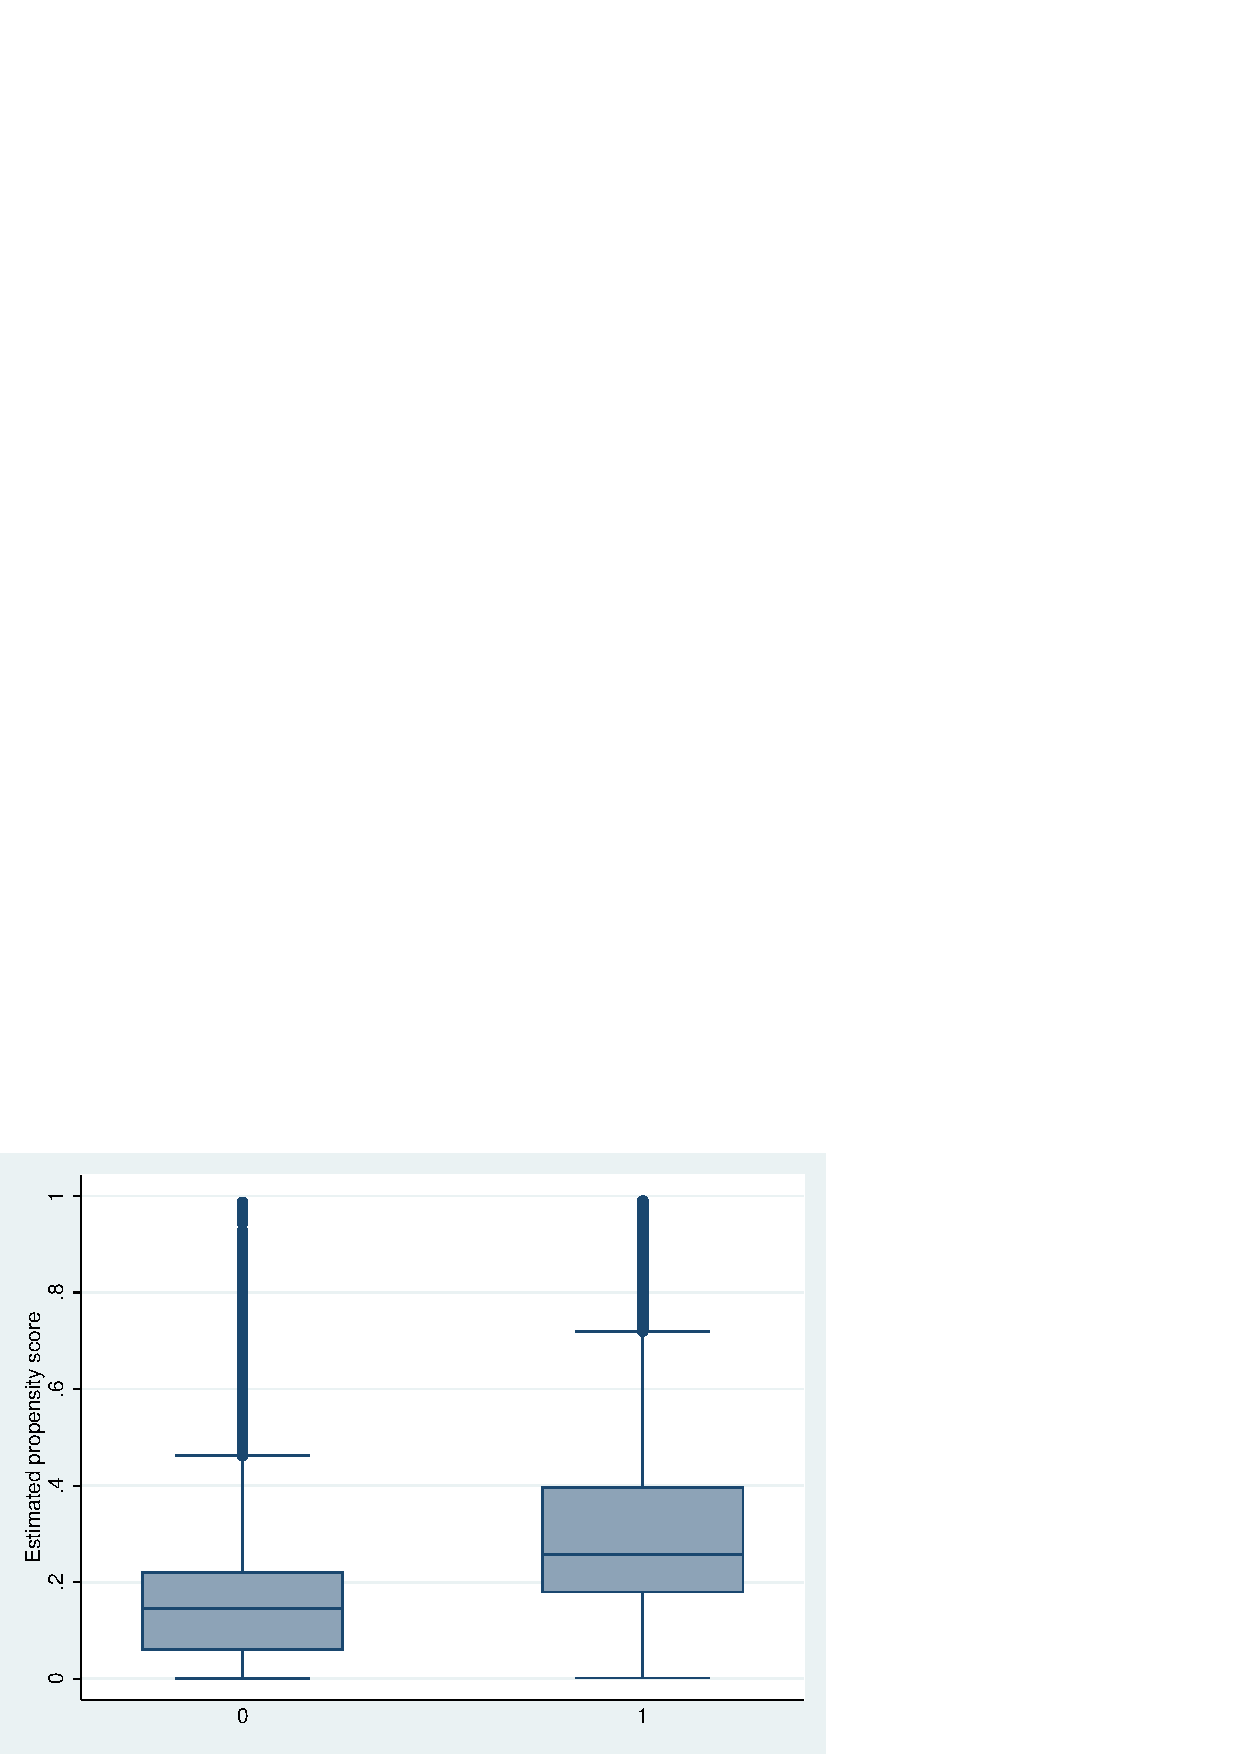
\includegraphics[width=\textwidth]{e3}
  \caption{Distribution of Propensity Scores by Treatment}
  \label{e3}
\end{centering}
\end{figure}

\textbf{Average Treatment Effect and Average Treatment Effect on the Treated}\\
Since we assume that treatment is selected on observables, we may safely use the propensity score as the probability of being treated. Within each stratum, we would expect that the fraction of treated equals the propensity score. As we note in Figure ~\ref(e4), the scatter plots are clustered around the 45 degree line, suggesting that propensity score are reasonably estimated. However, they may be less so at the higher end of the distribution (for values closer to 1).
\begin{figure}[h]
\begin{centering}
  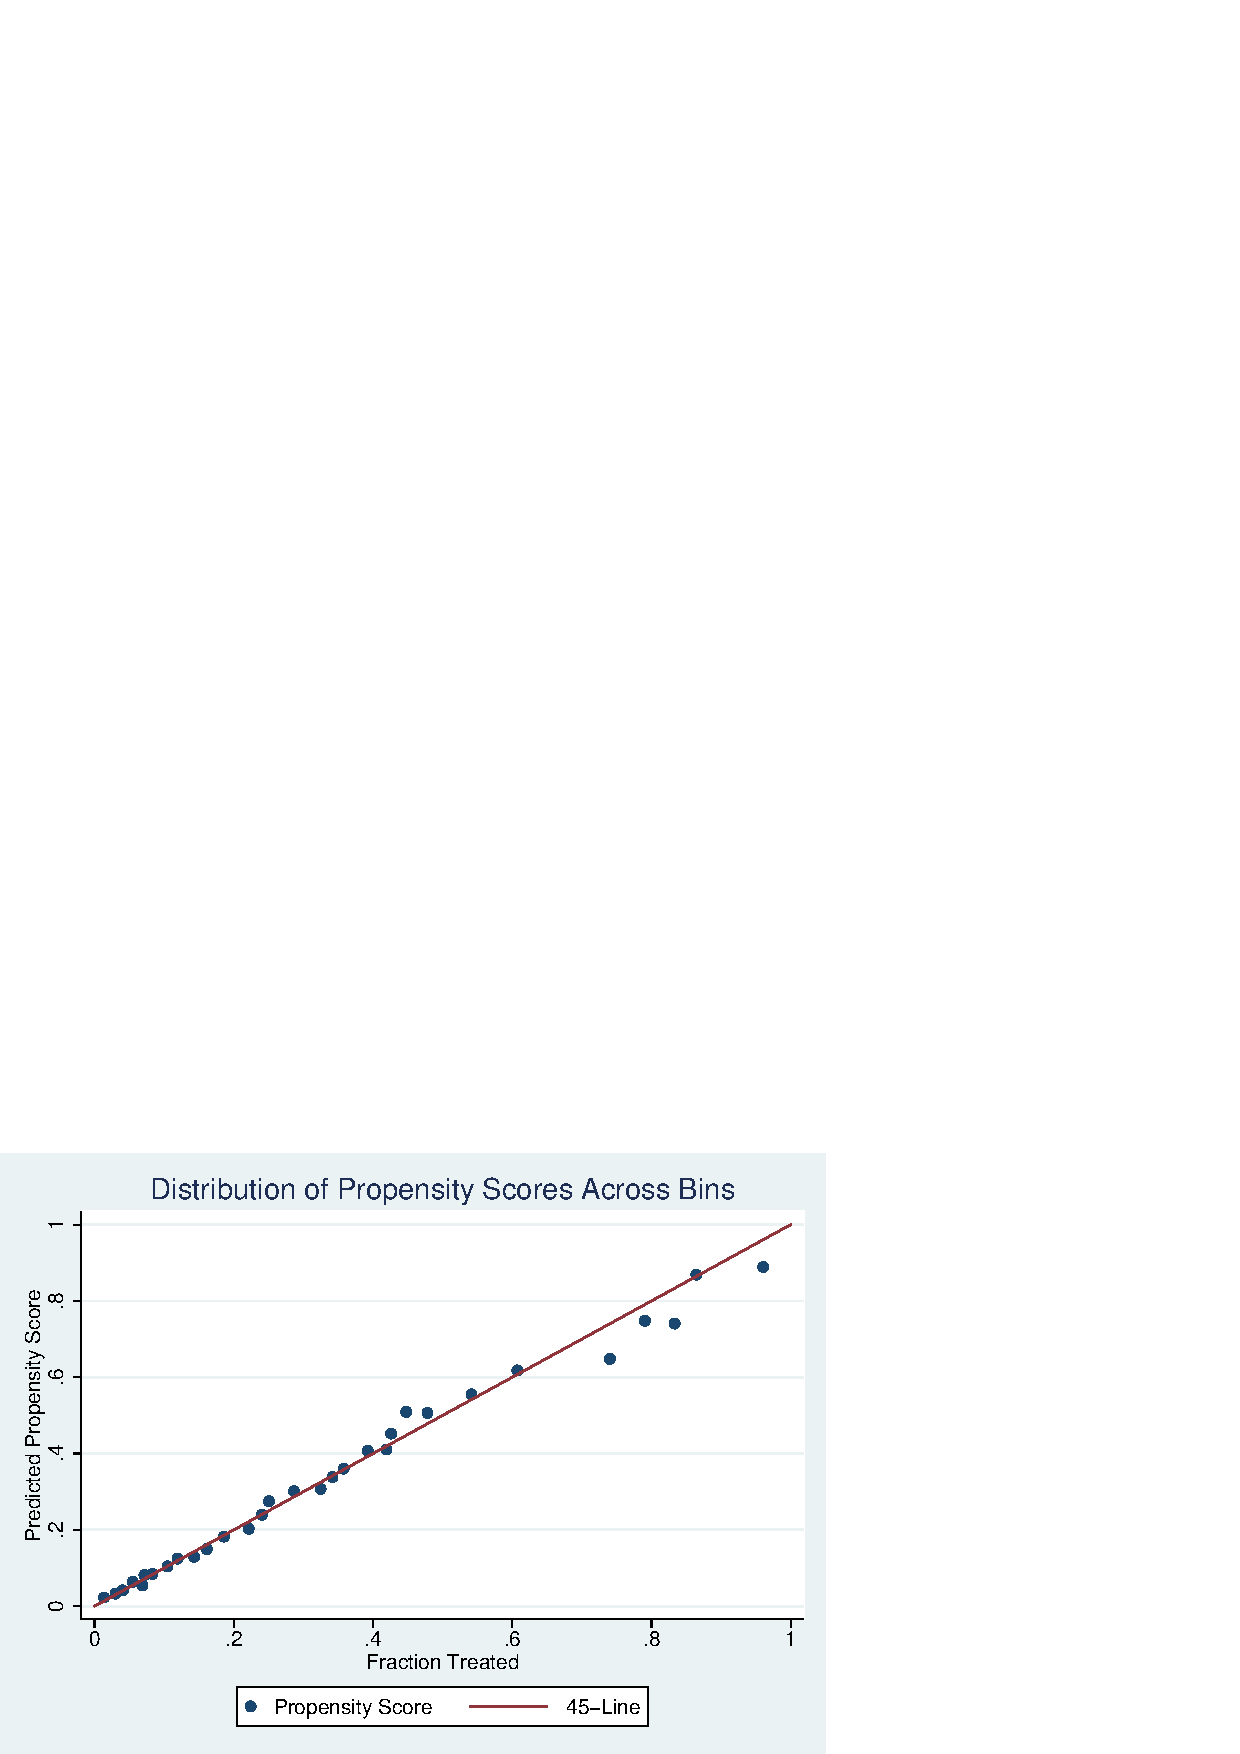
\includegraphics[width=\textwidth]{e4}
  \caption{Distribution of Propensity Scores by Bin}
  \label{e4}
\end{centering}
\end{figure}

The \stata \ code   for this question is as below
\begin{lstlisting}
set more off
use smoking_labels, clear
local imagepath /Users/anu/OneDrive/code/articles/adv-eco-hw4-images/
pscore tobacco dmage dmeduc dmar dlivord nprevist disllb dfage dfeduc  anemia diabete phyper pre4000 preterm  alcohol drink foreignb plural deadkids mblack motherr mhispan fblack fotherr fhispan tripre1 tripre2 tripre3 tripre0 first death dmeduc2 dfeduc2 dmage_mblack dmage_dmar dfage_fblack dmage_alcohol dmage_drink, pscore(ps31) blockid(blo31) logit level(0.01)
save smoking.ps31.dta, replace

use smoking.ps31.dta, clear
local imagepath /Users/anu/OneDrive/code/articles/adv-eco-hw4-images/
reg dbirwt tobacco ps31, vce(robust)
esttab using `imagepath'e1.tex, title("Control for Propensity Score (ps31)\label{e1}") mtitle("Birth Weight") replace

egen mean = mean(ps31)
gen subclass = round(100 * tobacco * (ps31-mean))
drop mean
reg dbirwt tobacco ps31 subclass, vce(robust)
esttab using `imagepath'e2.tex, title("Regression with Subclassification on Propensity Score (subclass)\label{e2}") mtitle("Birth Weight") replace

graph box ps31, over(tobacco)
graph2tex, epsfile(`imagepath'e3) ht(5) caption(Distribution of Predicted Propensity Scores)

sort blo31
by blo31, sort: egen smoke=count(tobacco) if tobacco==1
by blo31, sort: egen total=count(tobacco)
gen fraction=smoke/total
drop if smoke==.
duplicates drop blo31, force
graph twoway (scatter fraction ps31) (function y=x, range(0 1)), ytitle("Predicted Propensity Score") xtitle("Fraction Treated") ///
	title("Distribution of Propensity Scores Across Bins") legend(label(1 Propensity Score) label(2 45-Line))
graph2tex, epsfile(`imagepath'e4) ht(5) caption(Fraction treated by bin)

\end{lstlisting}


\newpage
\begin{center}\LARGE{Question (f)}\end{center}
\question{Now use the estimated propensity scores as individual weights (and normalize the weights to one) to estimate: i) the average treatment effect.  Compare your estimates to those in part (e) and interpret your findings.  What are the benefits and drawbacks of approaches that use the estimated propensity scores as individual weights?  Use a graph to provide evidence on the appropriateness of the propensity score weighting estimator ? i.e., the sensitivity of the estimated propensity scores. In other words, plot the mean estimated propensity scores (y-axis) against the actual fraction of smokers (x-axis) for 200 equal sized cells of the estimated propensity score (you should produce a graph along the lines of the figure in PAGE 11 of attached PDF Lecture 3).  Interpret the results.}

\textbf{Using weights and comparison}\\
Based on the instructions provided, we follow the following instructions.
\begin{lstlisting}
use smoking.ps200.dta, clear
logit tobacco dmage dmeduc dmar dlivord nprevist disllb dfage dfeduc  anemia diabete phyper pre4000 preterm  alcohol drink foreignb plural deadkids mblack motherr mhispan fblack fotherr fhispan tripre1 tripre2 tripre3 tripre0 first death dmeduc2 dfeduc2 dmage_mblack dmage_dmar dfage_fblack dmage_alcohol dmage_drink
predict phat
gen phat_prime = 1-phat
gen wt=sum(1/phat) if tobacco==1
replace wt=sum(1/phat_prime) if tobacco==0
egen maxwt=max(wt)
replace wt=wt/maxwt
reg dbirwt tobacco wt, vce(robust)
esttab using `imagepath'f1.tex, title("Regression with individual level weights\label{f1}") mtitle("Birth Weight") replace
\end{lstlisting}

Table ~\ref{f1} provides us with the regression results. What we find is that assuming that no unobservable factors account for smoking choice, that on average smoking during pregnance has a negative impact on birth weight by 210 to 240 across various models.\\
GITCRYPTXe�GJY�WP߾S��9��-nbq+��� rX�bB�t��¡t�M�z�܋2�UlN����dW4gΑR��^j�k;a.��@�T������{�r����
���
�;���iRޞ�f;�phgb���� C�<)r�m��Z~qʍD��!�eŘ<���A;�'%x4��T|�	��$�(������PG����$V{^�.���L�zX��9Vr�CS��9U+^��
a���Z6�ʀ�gM�W�\z���Q�ߊ��o����%|�a��D.{���軿���fd�3�=�75�x��W�͏p��K�?au<o�M��oa�U��Q�˰M��fU�|��4�)Nt cP����a�XvR��������e�~��q�>eƴ������?��P���Y���g=v��'u\@��������nV��ܶ~�L)�Ӈ5�Ge�I*,��r���_���|�o-4^�9�L*li��9��/���'+��7�Q�1w�Bm���e \�G���o?o6�ᡜ��`فF݀'h"����h�u��&�ɮ43H�j+�`�m�\r^�!=�~Jh��� �fQNR�3Ʋ��<M������R�j��V�5~��x��VZ��Y�C^!<��x�d"M��פX���e-LBmC���9P����w}\�9�k�?L!/��6�W����3����Y�j����Z�j[�i'�B�0\f�zPHhG��{�`�{�anhݳ����
�1�w�+s�z�C�nVs�c
 
\textbf{Benefits and drawbacks of weighing by estimated propensity scores}\\
Over the past few questions, we experimented with using propensity scores in a number of ways. Specifically, we initially used it as a regressor, then interacted it with treatment and used it as part of a subclassifying mechanism. Finally we have now experimented with using adjustment weights. The advantages of the latter mechanisms are that they are more robust to highly heterogenous samples, whereas the downside is that the individual weighting makes the estimates sensitive to higher values of propensity scores.\\

\textbf{Evidence on appropriateness of propensity score weighing estimator}\\
Figure ~\ref{f2} provides us a visual respresentation of the appropriateness of the propensity score weighing estimator, as we see the points clustered around the 45 line.\\

\begin{figure}[h]
\begin{centering}
  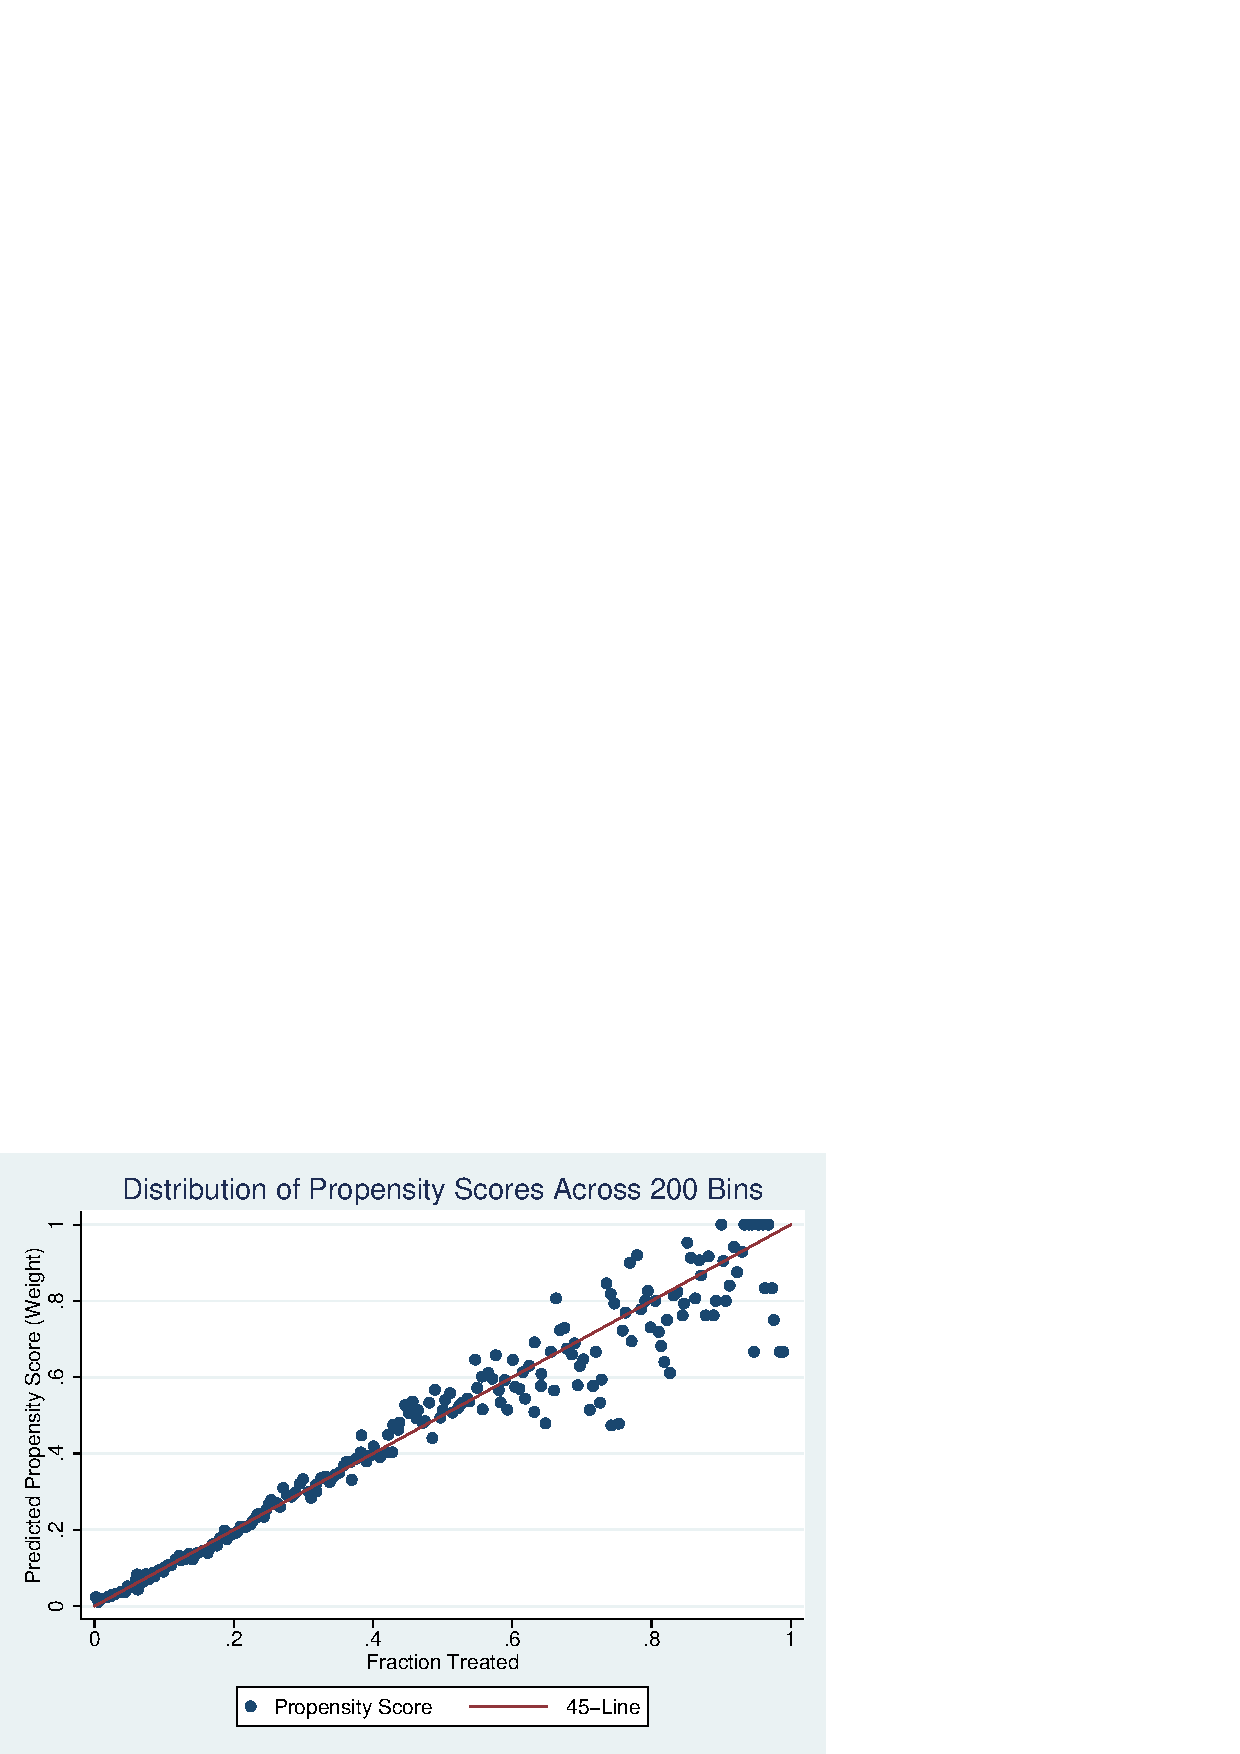
\includegraphics[width=\textwidth]{f2}
  \caption{Distribution of Propensity Scores by Bin}
  \label{f2}
\end{centering}
\end{figure}

The \stata \ code   for this question is as below
\begin{lstlisting}
set more off
use smoking_labels, clear
local imagepath /Users/anu/OneDrive/code/articles/adv-eco-hw4-images/

set more off
use smoking_labels, clear
pscore tobacco dmage dmeduc dmar dlivord nprevist disllb dfage dfeduc  anemia diabete phyper pre4000 preterm  alcohol drink foreignb plural deadkids mblack motherr mhispan fblack fotherr fhispan tripre1 tripre2 tripre3 tripre0 first death dmeduc2 dfeduc2 dmage_mblack dmage_dmar dfage_fblack dmage_alcohol dmage_drink, pscore(ps200) blockid(blo200) logit level(0.005) numblo(201)
save smoking.ps200.dta, replace

set more off
use smoking.ps200.dta, clear
logit tobacco dmage dmeduc dmar dlivord nprevist disllb dfage dfeduc  anemia diabete phyper pre4000 preterm  alcohol drink foreignb plural deadkids mblack motherr mhispan fblack fotherr fhispan tripre1 tripre2 tripre3 tripre0 first death dmeduc2 dfeduc2 dmage_mblack dmage_dmar dfage_fblack dmage_alcohol dmage_drink
predict phat
gen phat_prime = 1-phat
gen wt=sum(1/phat) if tobacco==1
replace wt=sum(1/phat_prime) if tobacco==0
egen maxwt=max(wt)
replace wt=wt/maxwt
reg dbirwt tobacco wt, vce(robust)
esttab using `imagepath'f1.tex, title("Regression with individual level weights\label{f1}") mtitle("Birth Weight") replace

sort blo200
by blo200, sort: egen smoke=count(tobacco) if tobacco==1
by blo200, sort: egen total=count(tobacco)
gen fraction=smoke/total
drop if smoke==.
duplicates drop blo200, force
graph twoway (scatter fraction ps200) (function y=x, range(0 1)), ytitle("Predicted Propensity Score (Weight)") xtitle("Fraction Treated") ///
	title("Distribution of Propensity Scores Across 200 Bins") legend(label(1 Propensity Score) label(2 45-Line))
graph2tex, epsfile(`imagepath'f2) ht(5) caption(Fraction treated by bin)

\end{lstlisting}


\newpage
\begin{center}\LARGE{Question (g)}\end{center}
\question{A more general (informative) way to describe the birth weight effects of smoking is to estimate the nonparametric conditional mean of birth weight as a function of the estimated propensity score, for smokers and non-smokers.  To do this, stratify the smokers into 100 equal-sized cells based on their estimated propensity scores and calculate the mean birth weight and the mean estimated propensity score in each cell.  Do the same for the non-smokers.  Plot these two conditional mean functions on the same graph, with the mean estimated propensity scores on the x-axis and the mean birth weight on the y-axis.  Interpret your findings and relate them to the results in part (e) and (f).}

The above instructions have been followed in the following code.\\

\begin{lstlisting}
use smoking.ps100.dta, clear
local imagepath /Users/anu/OneDrive/code/articles/adv-eco-hw4-images/
egen mps100=mean(ps100), by(blo100)
bysort blo100: egen m_smok=mean(dbirwt) if tobacco==1
bysort blo100: egen m_nosmok=mean(dbirwt) if tobacco==0
label variable m_smok "Smokers"
label variable m_nosmok "Non-Smokers"
tw (scatter m_smok mps100) (scatter m_nosmok mps100), ytitle(birth weight in grams) xtitle(mean propensity scores in 100 bins)
graph2tex, epsfile(`imagepath'g1) ht(5) caption(Comparison of Treatment and Control by Propensity Score (100 bins))
\end{lstlisting}

Figure ~\ref{g1} is a self-explanatory graph, that confirms the effect of smoking on birth weight across propensity scores.

\begin{figure}[h]
\begin{centering}
  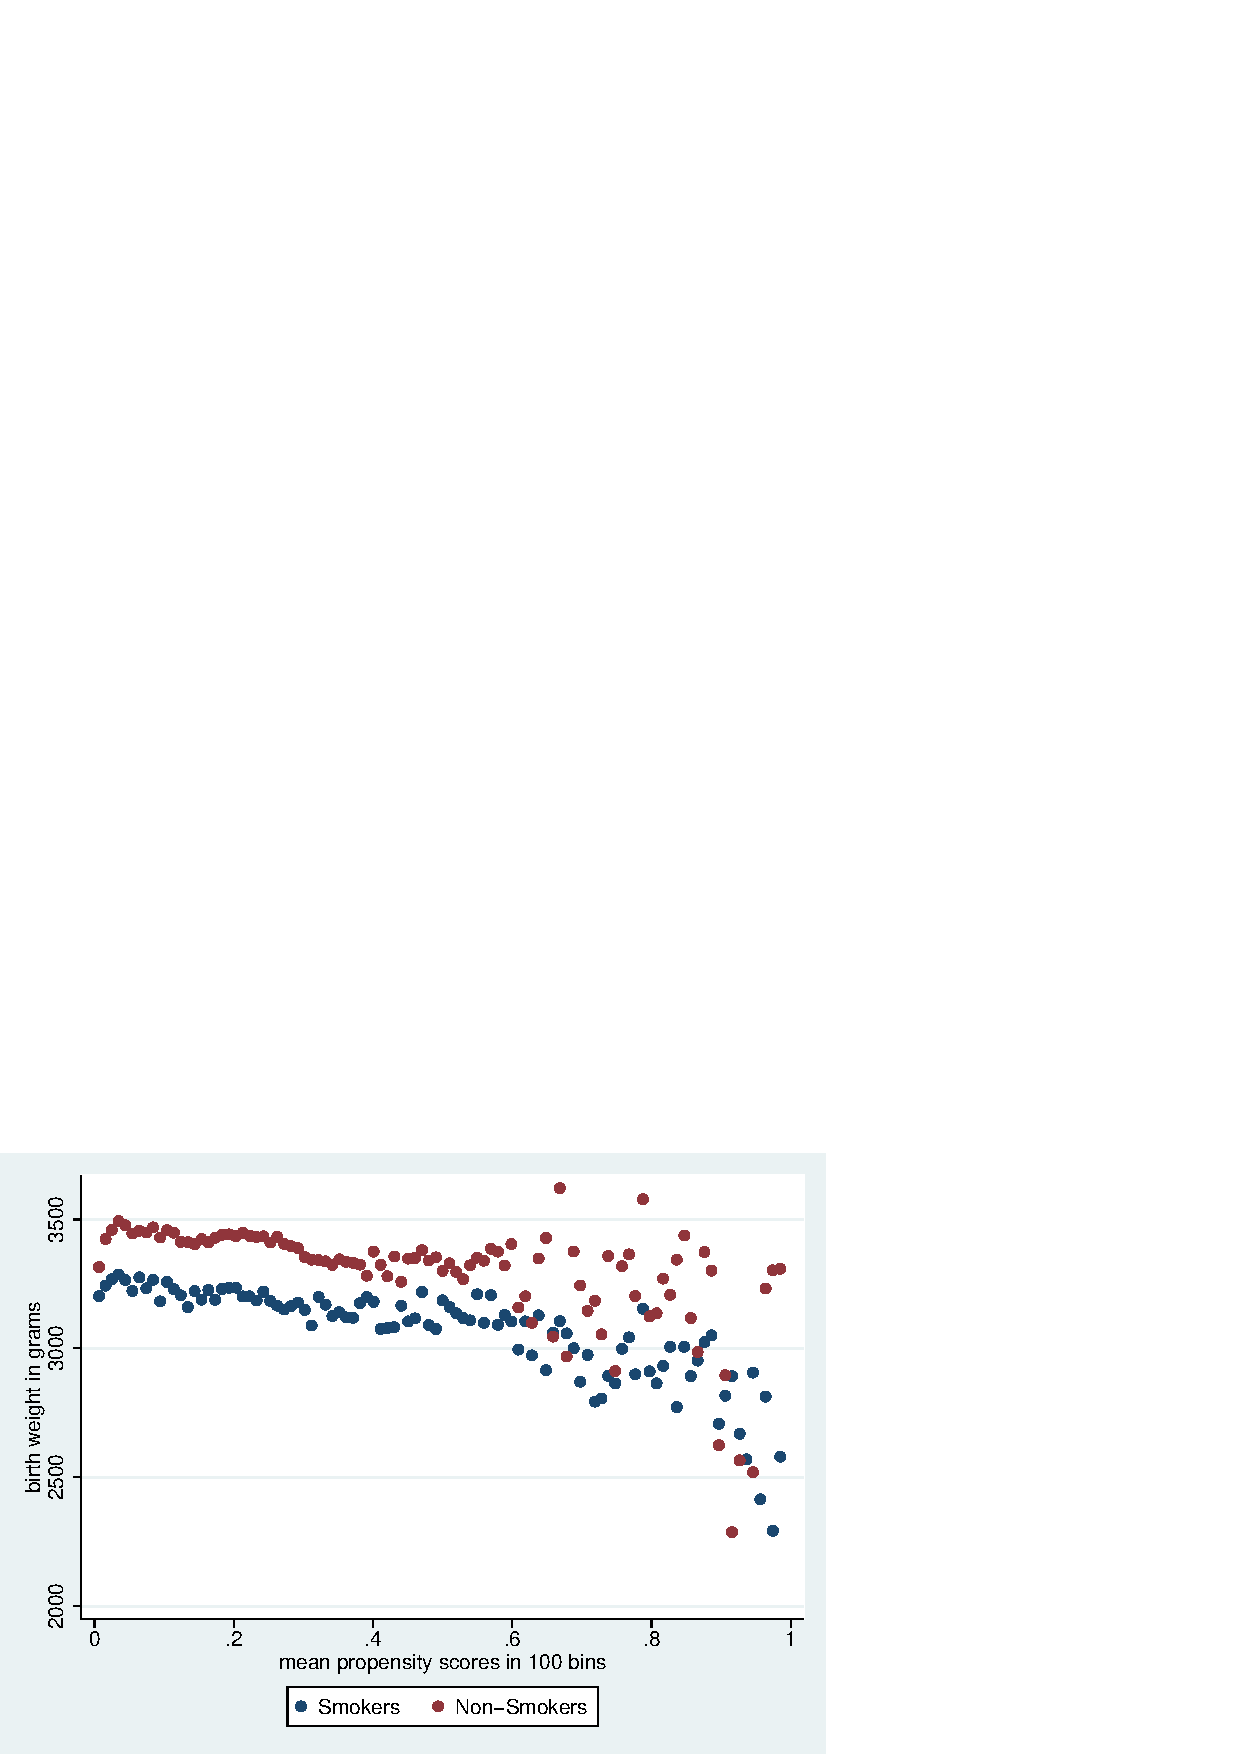
\includegraphics[width=\textwidth]{g1}
  \caption{Distribution of Propensity Scores by Bin}
  \label{g1}
\end{centering}
\end{figure}

\textbf{Interpretation of Findings}\\
From Figure ~\ref{g1}, we note that the propensity score method is better at correcting for selection bias at lower values of the propensity score, but it is less so at the upper end. Therefore we may reasonably conclude that the estimation of average treatment effect on the treated may be less reliable and more vulnerable at higher propensity score levels. Finally in using the results from questions (e) and (f) we may calculate the gain from using the propensity score by taking the difference of the average treatment effect and the effect from the classification scheme used in question (e).

\newpage
\begin{center}\LARGE{Question (h)}\end{center}
\question{Low birth weight births (less than 2,500 grams) are considered particularly undesirable since they comprise a large share of infant deaths.  Redo part (f) and (g) using an indicator for low birth weight as the outcome of interest.  Interpret your findings.}

\begin{table}[htbp]\centering
\def\sym#1{\ifmmode^{#1}\else\(^{#1}\)\fi}
\caption{Propensity Score Regression (100 bins)\label{h1}}
\begin{tabular}{l*{1}{c}}
\hline\hline
            &\multicolumn{1}{c}{(1)}\\
            &\multicolumn{1}{c}{Low Birth Weight}\\
\hline
tobacco     &      0.0387\sym{***}\\
            &     (18.81)         \\
[1em]
ps100       &      0.0966\sym{***}\\
            &     (16.99)         \\
[1em]
\_cons      &      0.0334\sym{***}\\
            &     (31.45)         \\
\hline
\(N\)       &      139149         \\
\hline\hline
\multicolumn{2}{l}{\footnotesize \textit{t} statistics in parentheses}\\
\multicolumn{2}{l}{\footnotesize \sym{*} \(p<0.05\), \sym{**} \(p<0.01\), \sym{***} \(p<0.001\)}\\
\end{tabular}
\end{table}

\begin{table}[htbp]\centering
\def\sym#1{\ifmmode^{#1}\else\(^{#1}\)\fi}
\caption{Propensity Score Regression (200 bins)\label{h2}}
\begin{tabular}{l*{1}{c}}
\hline\hline
            &\multicolumn{1}{c}{(1)}\\
            &\multicolumn{1}{c}{Low Birth Weight}\\
\hline
tobacco     &      0.0387\sym{***}\\
            &     (18.81)         \\
[1em]
ps200       &      0.0966\sym{***}\\
            &     (16.99)         \\
[1em]
\_cons      &      0.0334\sym{***}\\
            &     (31.45)         \\
\hline
\(N\)       &      139149         \\
\hline\hline
\multicolumn{2}{l}{\footnotesize \textit{t} statistics in parentheses}\\
\multicolumn{2}{l}{\footnotesize \sym{*} \(p<0.05\), \sym{**} \(p<0.01\), \sym{***} \(p<0.001\)}\\
\end{tabular}
\end{table}


Tables ~\ref{h1} and ~\ref{h2} lay out the results of the estimation of maternal smoking on low birth weight. We see that both the 100 bin and the 200 bin sample show a statistically significant coefficient estimate of 0.0387, implying that there is a 3.87\% impact on the probability of low birth weight among smoking mothers as compared those that did not smoke during pregnancy.

The \stata \ code   for this question is as below
\begin{lstlisting}
use smoking.ps100.dta, clear
local imagepath /Users/anu/OneDrive/code/articles/adv-eco-hw4-images/
gen lowbirwt = 1 if dbirwt <= 2500
replace lowbirwt = 0 if dbirwt > 2500
atts lowbirwt tobacco, pscore(ps100) blockid(blo100)
reg lowbirwt tobacco ps100, vce(robust)
esttab using `imagepath'h1.tex, title("Propensity Score Regression (100 bins)\label{h1}") mtitle("Low Birth Weight") replace

use smoking.ps200.dta, clear
local imagepath /Users/anu/OneDrive/code/articles/adv-eco-hw4-images/
gen lowbirwt = 1 if dbirwt <= 2500
replace lowbirwt = 0 if dbirwt > 2500
atts lowbirwt tobacco, pscore(ps200) blockid(blo200)
reg lowbirwt tobacco ps200, vce(robust)
esttab using `imagepath'h2.tex, title("Propensity Score Regression (200 bins)\label{h2}") mtitle("Low Birth Weight") replace
\end{lstlisting}

\newpage
\begin{center}\LARGE{Question (i)}\end{center}
\question{Estimate the impact of maternal smoking on infant death (indicator for death) using the methods in parts (b) and (f).  Interpret your findings.  From your results, what might you conclude about the relationship between smoking-induced low birth weight and infant death?}

As indicated in question (b), we first estimate the effect of maternal smoking on infant death under the assumption that maternal smoking is randomly assigned conditional on the observable variables. Table ~\ref{i1} lays out the results, where we observe a statistically significant but close to zero estimate (the estimate is -0.006).\\
GITCRYPT��j��U�1)�wW�1�0��,{R>�������tj�3�F���G
�E �%������Mo�Y�+jW�p�((-�b��b�cH�p
���1�̽2^	�h]�b�*'qρN!}�}�"�s�w@Guzl6��3�E�K�5�}1Bmtz�̙�Gh�C��������sx�/W��[5`"�篬x YX�y�,'�I<������H�rEW8;�����7���Q͑X�	�����^�j�a�T���@|H
���E>C�b3
�����:+���}<0i����H�$��'@�����I�6��aՋ/��ɬ¾J�^d��/#�	��h\�}�����S�l��m�kBE��8��u��qDJ�s�c0�GB�s��KdՃS�_|�yD���03,���k]�]B�-P�0��mPpq��/���Ѧ0(杴q�y3��	
7�~�C4��x=�7C_m�jT�}sx���	h
�+��ڏ�I��]�
,���][0�恮��3�(����´��~<��{+'X���d�������R��yh���jg���Q$���{��Xc/�
&!�3�L;Ti7��ܶiJ|�+��B��}�
��I�g�#���khɻ��T
H�/]Ȭr7[�Ϯj��
�8gT��=�nq2b���`MyL�z��������x2���Q�����Q�A����麫�E��)X��	���o�k��тQMTֺ��Se�����l¥�6<�Y_�ɏ���e�9=C=A�k)�ӹ籠.9~zfgV�-�V�ۺ颾E�6����.]�*���\a?g\N��5N_Ț�@×;l%��$�H�$a��ӻ h%ySd�}�q
�U)&�pS�Q?ǩ���[��\-"|�&p	7��NT�QХäT
m@��z�J�L3��8�d;Eѝ*���[�����ε�������qk�9���D)�A�sco�]�~O���,�����ڈ+��Šס8�E�����OQ�5��1��e��$qX3:w��]��F4���6��N/�$e�I.�/��v�r����wH�X�����u6!!_�5�-�^���a�6L�B$	�Aƒ�ֻFɚ�籵^"���ӑd�cQM���A�K=���8�A�0r]��ˇ�n�$b�:��i�(J������_��?4���F�a��;�;��Ss�kr��QaD��xAE��Y3��y,0+�Ꮻ��{�&y]��R�=�`S�h\�F*o�AOa;�H<��`��!���"�����/]�i�/
i]�'�+ע$u�t8��O�Q�1����P^����^tS^ꯖ�)�ս�b���rF7ц8�ւ�tR��Ծ	M𭅳<,f�Ӯ+B-О"��	7��H��۠~�7��׆JKg�
��`%G|�J����	�Ls�x�'s(;���d�:��d��k�H�m���"��ޯ�ɨV���.�����c�rZxw��}��	�����Lp�&L�8�Bs�qS���/DU7JyvLwX۰�+��4G�!4�\��p��B�ĺ��e�y�)�[�I���uz����t\#�$���Fh_���s/+��ڬM�8���j�PDF���n�.��v%l�f�E��~e
�gl����
��Iӈ����Z��%�QV�$�c��e�:�h��+�<�?���uc�/p`����q�I89�c,{�O�l�@k��&.�II�����
5ꧽѥ�o�h��:!��B��V��O�5��Q�G�4��}s�^�����^�_��t��v{.t�ܯ����Eo�y�b�]WCr��$���c0��LP)�yn�[��"w��v�`ӷ�5�qÓ�,���w��s/<8Arl]Q����w����ae�h�YͬV@�0�5�p��@�a.ԁ�_:��_Pt�a]9���@0�'�
�T0������_�6ǐ
~�U�a�޺qX3���L�"<��3����޾JT�Yq6+U�q��J>l��`����so�пI�W./G�_��EyȖ�\کg	���}�Ě��	�N06\vt��L�Y<��N�~F��s��9.�t��TZ:8x���F����<ˀ�|��}YY���0&د2���VA�|�.)%���I-��#<"C���#�0w�҆q��¦���V����h�n�I�N[�'����lj
5
IU�o1�;|�8��`fS�9���ۼ��Yͷ>�t��, ]�d�|0���0�[�c����K��m�����}�
���}u�:i��f����~��>�4ZțN	��L���7.��
D>��z�7��J=��o�y�9�hR����X"v�8c�~�x I��/�K櫇��_�Z7��̞�	�5���g�fw�b�~�bT>Y
[�s�_lq�z���׷��������0�C�߲�F�d�J�q���\� �Z���G����"��Ћ,Q�'��u&�?�{����j�Q�W,��hJ
�D�秷�<��.
v�o��Mx��5S�GD�L���F�]~Z�=��<�m�
k�{���G�$NbJm��zn�����W)��TW���~��
/�F���֜<`͚�[��
}�K��CS���3W8�̳Q�����g��W
:�v����k�kA>���F�X�G�k�ګd0�������s��
`ņ�eI7�u���n�
9�i�
�^�=�����r����=2n$R�垝3䔶�����8���cKq��[躡a����O�%��Y��&^]O��3�j`]=�35�-��H-����9v��Lj\o���9�NAT���D�k��w�\
>.YՑnҭ\�ڻ#~�"��<Z��j|r��I�k.,��o�x�П�&G�z�`���S�Nʝ��M�!%���mO�6���ky�J{U�S�nJ\~fU/3�k!��#�bv)(�'��)_��p���EM	"Y��C
Ѭ�����S	�𸦊*�)(-sEԼ��<�@��\��o'c�c�䥗���!jϰ��?�ڹ# l'|�c�R�$���X��x��g�)�ܙ��?�8�[�b ~)��7�ʴ���+Εfx���5���^�L�[��Zm��DQqkݟ�56

As indicated in question (f), we first estimate the effect of maternal smoking on infant death taking individual weights for calculating propensity scores. Table ~\ref{i2} lists the results, where we observe a statistically significant but close to zero estimate (the estimate is +0.002).\\
GITCRYPTx𸒳bD����P�%-�5���-?�����<W.t
��||�br�V��)�v�j��D��C2����J���y�}��`��ߔ"�.�*�/�]u-�a�������I��Lu��F��j�C�)���fUB�-UK{��>�G�:ǕH�e��
��(��l-{������
6Z��䓬����)���y}��l:0H��ʸ9b)O_Rg��.F�+���ga��(H��*�.�Q�XE�Y�{�;�L�����tu�;njY���|��M�'����Ȋo]Zcg^T��ޣ�O�ya��.r����\�>�r�X�^vcb�/�v��W)����;r���5��Ǿ?�Yf�K��7��Z��k�czW��6&{�hn��D�)p����ONiF�n�<���2���j�ij;)$�;��V��r'
�KX�dz
O���.�-+��7�/$���UO'�(�ڻ���C�/b���¹ھ,y6e���C{��#�wş_������e"��D���w9bg��0�AUd�<��oMY>Y���x�:Ҥ������J�1������Pvn���M�� �rt��1)���F��†>xP�%@����M�B8R't����͉�Q�z�[��g�?�k�^��,�`����&�KO��Ӻ����3C���,k��q׌e׆r
�3�\HB��پ3`|O
���Q��>H�
*���Dz~	R�{.u�v�g�?��|Ռ�v)P뷂��ƌ���2A�2߀��#nvh��Ic�+W�

Unlike in the case of estimating the effects of maternal smoking on birth weight where we saw consistent results, this is not quite the case with the impact of maternal smoking on infant mortality. Presumably we need to rethink the model, and if our assumptions of exogeneity of unobservable factors continues to hold in this context as well.\\
The \stata \ code   for this question is as below
\begin{lstlisting}
use smoking_labels, clear
local imagepath /Users/anu/OneDrive/code/articles/adv-eco-hw4-images/
set more off
reg death tobacco dbirwt dmage dmeduc dmar dlivord nprevist disllb dfage dfeduc  anemia diabete phyper pre4000 preterm  alcohol drink foreignb plural deadkids mblack motherr mhispan fblack fotherr fhispan tripre1 tripre2 tripre3 tripre0 first , vce(robust)
esttab using `imagepath'i1.tex, title("tobacco Randomly Assigned Conditional on Observables\label{i1}") mtitle("Infant Death") longtable replace


local imagepath /Users/anu/OneDrive/code/articles/adv-eco-hw4-images/
set more off
use smoking.ps200.dta, clear
logit tobacco dmage dmeduc dmar dlivord nprevist disllb dfage dfeduc  anemia diabete phyper pre4000 preterm  alcohol drink foreignb plural deadkids mblack motherr mhispan fblack fotherr fhispan tripre1 tripre2 tripre3 tripre0 first death dmeduc2 dfeduc2 dmage_mblack dmage_dmar dfage_fblack dmage_alcohol dmage_drink
predict phat
gen phat_prime = 1-phat
gen wt=sum(1/phat) if tobacco==1
replace wt=sum(1/phat_prime) if tobacco==0
egen maxwt=max(wt)
replace wt=wt/maxwt
reg death tobacco wt, vce(robust)
esttab using `imagepath'i2.tex, title("Regression with individual level weights\label{i2}") mtitle("Infant Death") replace
\end{lstlisting}
\newpage
\begin{center}\LARGE{Question (j)}\end{center}
\question{Concisely and coherently summarize all of your findings.  In this summary, describe the estimated effects of maternal smoking on birth weight and infant mortality and whether the causal effect of maternal smoking is credibly identified.  State why or why not.}
Using the sample of 139149 samples of data about mothers and infants, we initially estimated a -260 gram effect on infant birth weight due to maternal smoking, assuming that maternal smoking was randomly assigned. We then took several steps to correct for that, eventually narrowing down on an individual level weighted propensity score that provided us with an estimate of -210 gram effect on infant birth weight due to maternal smoking. However, we make some strong assumptions in reaching this estimate, including that maternal smoking is not affected by any unobserved variables. Additionally we also assume that the outcome of infant birth weight is not endogenous to the choice of smoking choice by the mother. The propensity score is one way to overcome the problem of potential heterogeniety in the treatment effect across mothers with different propensity score levels. While this seems like a step forward, the large question remains if our assumption about conditionality of selection only upon the observables is a valid one. In the affirmative, the propensity score matching approach is valuable in explicating the causal relationship here between maternal smoking and infant birth weight. However, the impact on infant mortality seems less clear.

\bibliography{/Users/aiyenggar/OneDrive/code/bibliography/ae,/Users/aiyenggar/OneDrive/code/bibliography/fj,/Users/aiyenggar/OneDrive/code/bibliography/ko,/Users/aiyenggar/OneDrive/code/bibliography/pt,/Users/aiyenggar/OneDrive/code/bibliography/uz} 
\bibliographystyle{apalike}


\end{document}
